\documentclass[11pt]{report} % { book | article | report }
% -------------------- Langue --------------------
\usepackage[utf8]{inputenc}
\usepackage[T1]{fontenc}
\usepackage[francais]{babel}
% -------------------- Marges, interlignes--------------------
\usepackage[a4paper]{geometry}	% 
%\usepackage{setspace}
%\usepackage{layout}		% Layout
%\usepackage{lscape}		% Orientation de la page
% -------------------- Soulignement --------------------
%\usepackage{soul}
%\usepackage{ulem}
% -------------------- Fontes --------------------
%\usepackage{eurosym}		% Symbole Euro
%\usepackage{bookman}
%\usepackage{charter}
%\usepackage{newcent}
%\usepackage{lmodern}
\usepackage{mathpazo}					
%\usepackage{mathptmx}
% -------------------- Code et citations --------------------
%\usepackage{verbatim}		% Code
%\usepackage{listings}		% Code avec coloration syntaxique
%\usepackage{url}		% Urls
%\usepackage{moreverb}
% -------------------- Couleur --------------------
%\usepackage{color}		% les couleurs
%\usepackage{colortbl}		% les couleurs dans un tableau
%\usepackage[svgnames]{xcolor}	% le package color, en mieux !
% -------------------- Maths --------------------
%\usepackage{amsmath}
%\usepackage{amssymb}
%\usepackage{mathrsfs}
%\usepackage{asmthm}
% -------------------- Images --------------------
\usepackage{graphicx}		% Insertion d'images ou de pdf -> option : [pdftex]
\usepackage{wrapfig}		% Ins\'erer des images dans un paragraphe
\usepackage{float}		% Argument H des figures
% -------------------- Tableau --------------------
%\usepackage{multirow}		% Fusion de cellules sur plusieurs lignes -> multirow{nblign}{size}{texte}
% -------------------- Autres --------------------
%\usepackage{makeidx}		% Cr\'eation d'index
%\usepackage{fancyhdr}		% Personnalisation des entetes
%\usepackage{sfheaders}		% Mise sans-serif des titres
%\usepackage{enumitem}		% Personnalisation des environnement enumerate	
%\usepackage{pdfpages}
%\usepackage[nottoc, notlof, notlot]{tocbibind}
%\usepackage{tocvsec2}		% Donne le choix du d\'epart de la num\'erotation


% -- Avec le package listings
% \lstset{language=java}
% -- Avec le package tocvsec2 (dans le document)
% \maxsecnumdepth{chapter}



\begin{document}
\begin{titlepage}

\vspace*{1.5cm}

\Huge
\begin{center}
Plug-in multi-agent pour une plate-forme de simulation de mobilité urbaine
\end{center}

\vspace{2cm}



\Large
\begin{flushleft}
\item Étudiants : 
\item Barberot Mathieu
\item Racenet Joan
\end{flushleft}

\begin{flushleft}
\item Tuteurs : 
\item Lang Christophe
\item Marilleau Nicolas
\end{flushleft}

\vspace{2cm}

\begin{center}
\item \today
\item UFR ST - Besançon
\item 
\includegraphics[height=1cm]{images/logo-ufc.png}
\end{center}

\end{titlepage}
\tableofcontents
\newpage

\chapter{Simulation Urbaine}
Un syst\`eme multi-agents est, comme son nom l'indique, un ensemble d'agents (entit\'es autonomes dot\'ees d'une intelligence artificielle constitu\'ee de comportements pr\'ed\'efinis) capables d'interactions aussi bien entre eux, qu'avec leur environnement et capables de s'adapter en fonction de l'\'etat de celui-ci.\\
Les SMA (pour syst\`emes multi-agents) proposent donc une approche assez intuitive pour simuler des comportements \og de masse \fg - les premiers exemples qui nous viendraient rapidement en t\^ete seraient les jeux vid\'eos ou le cin\'ema, o\`u des effets sp\'eciaux mettant en sc\`ene une foule d'entit\'es peuvent \^etre simul\'es par un SMA de mani\`ere cr\'edible, \'evitant ainsi aux graphistes la tâche colossale d'animer et de coordonner des centaines, voire des milliers de mod\`eles 3D.\\
Mais outre son application \`a des syst\`emes purement virtuels, on s'aperçoit rapidement que la philosophie des SMA est particuli\`erement adapt\'e pour des simulations ayant pour contexte les sciences humaines. On s'int\'eressera plus particuli\`erement ici \`a une application au domaine de la simulation urbaine. Concr\`etement, il serait int\'eressant de pouvoir observer le comportement d'\^etres humains dans une ville et de pouvoir mesurer l'impact de certaines modifications de l'environnement sur ces derniers (par exemple, dans quelle mesure serait influenc\'e le trafic routier si j'entreprends des travaux sur tel ou tel axe).\\
C'est dans cette optique qu'a \'et\'e d\'evelopp\'e le projet MIRO qui consiste en une analyse des flux d'activit\'es quotidiennes (comme par exemple le trafic routier ou les mouvement des habitants en fonction de l'heure de la journ\'ee) de la ville de Dijon.Le projet tuteur\'e, dont nous allons ici d\'etailler les tenants et aboutissants, s'inscrit dans cette th\'ematique, \'etant donn\'e que son objectif est justement de fournir des outils pour simplifier au maximum l'\'ecriture d'une simulation de mobilit\'e urbaine.

\chapter{La plate-forme : GAMA}
\begin{wrapfigure}[20]{l}{0.45\textwidth}

\includegraphics[width=0.4\textwidth]{images/gaml-logo.png}%
\caption{GAMA}%
\end{wrapfigure}
Les outils dont nous venons justement de parler ont pour vis\'ee d'\^etre int\'egr\'es au sein de la plate-forme de d\'eveloppement de syst\`emes multi-agents nomm\'ee GAMA.\\
GAMA est un IDE (environnement de d\'eveloppement) open-source bas\'e sur Eclipse (donc cod\'e dans le langage Java) et d\'evelopp\'e par l'UMMISCO (Unit\'e de Mod\'elisation Math\'ematique et Informatique de Syst\`emes COmplexes) depuis 2007.\\
Cette plate-forme est tr\`es nettement orient\'ee g\'eomatique, puisqu'elle propose nativement des outils permettant d'exploiter des donn\'ees complexes issues de Syst\`emes d'Informations G\'eographiques (SIG ou GIS en anglais) afin de d\'efinir l'environnement des simulations (on pourra par exemple r\'ecup\'erer rapidement le trac\'e des routes d'une ville et ses bâtiments).\\
Pour l'\'ecriture des simulations, GAMA propose son propre langage nomm\'e GAML (pour GAMA Language), qui permet de manipuler facilement des agents, leur environnement ainsi que divers types complexes classiques (listes dynamiques, graphes …).\\
Les fonctionnalit\'es propos\'ees par GAMA sont impl\'ement\'ees au sein de plug-ins Eclipse venant se greffer autour du noyau de l'application. Afin de fournir nos propres fonctions, nous passerons nous-m\^emes par le d\'eveloppement d'un greffon en se basant sur la version d\'eveloppeur de GAMA, librement t\'el\'echargeable. Cette m\'ethode a l'avantage d'\'eviter aux \'eventuels d\'eveloppeurs de modifier la base de l'application.



\chapter{Pr\'esentation du plug-in}

\section{La mod\'elisation d'une ville avec GAMA}
\begin{figure}[!ht]%
\begin{center}
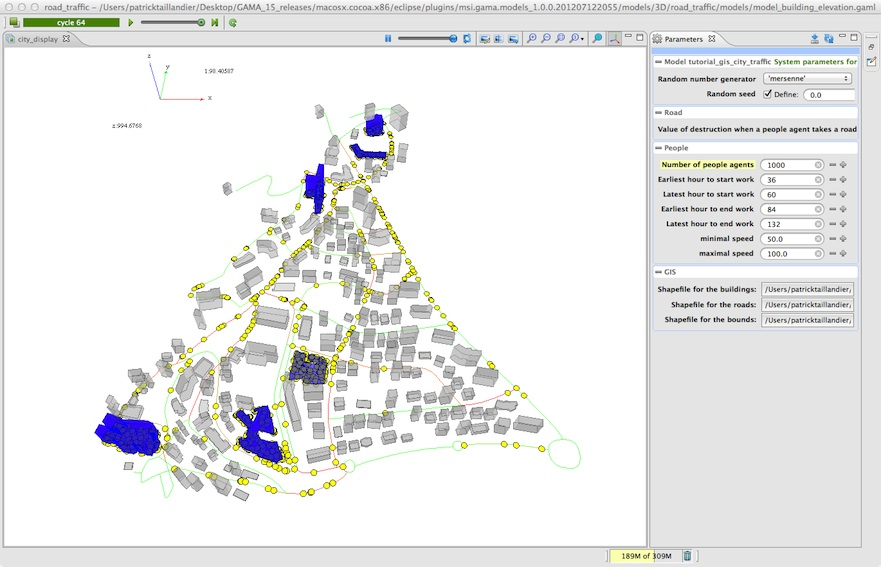
\includegraphics[width=\textwidth]{images/screenshot2.jpg}%
\end{center}
\caption{Mod\'elisation d'une ville}%
\end{figure}%
Comme on l'a vu, importer le trac\'e d'une ville, ses routes et ses bâtiments, est assez ais\'e dans GAMA, puisqu'on peut les importer directement depuis un SIG. De m\^eme, on peut rapidement exploiter ces donn\'ees, en les assignant \`a des types d'agents (dans notre cas, on pourra cr\'eer un agent pour les routes, un autre pour les bâtiments et enfin un dernier pour la population de la ville). Par la suite, nous pourrons cr\'eer un graphe en utilisant les routes en tant qu'ar\^etes et les \og services \fg{} (objectifs pour la population) en tant que n\oe{}uds afin de repr\'esenter la ville en m\'emoire. La ville pourra \^etre ensuite librement parcourue par les agents, ce que GAMA traduit par un parcours de graphe et l'application d'algorithmes de recherches des plus courts chemins (Dijkstra) dans le cas o\`u l'on cherche \`a faire atteindre un objectif \`a un agent.\\
Mod\'eliser la ville en elle-m\^eme est donc relativement ais\'ee. En revanche, les choses se compliquent rapidement d\`es que l'on veut donner des comportements r\'ealistes aux agents de la population, comme leur faire respecter le code de la route (par exemple, respecter les sens uniques ou les limitations de vitesse) ou leur faire subir les contraintes de l'environnement (r\'eduction de la vitesse en fonction du nombre d'autres automobilistes sur un tronçon). Cela reste possible, mais moyennant une certaine quantit\'e de code GAML suppl\'ementaire assez complexe.\\
Le but de notre plug-in est donc de rendre plus accessibles l'\'ecriture de simulation utilisant ce genre de comportements, en proposant nativement ceux-ci dans le logiciel au d\'eveloppeur GAML. Dans le cadre de notre travail, nous nous sommes concentr\'es justement sur le respect des sens uniques et des limitations de vitesse.

\section{Contenu du plugin}
La solution que nous avons trouv\'ee pour faciliter cette mod\'elisation est d'embarquer un agent pr\'ed\'efini repr\'esentant une rue, afin d'\'eviter aux utilisateurs de red\'efinir lui-m\^eme un tel type \`a chaque \'ecriture d'une nouvelle simulation. Pour simplifier leur utilisation, ces agents peuvent \^etre instanci\'es \`a l'importation d'un fichier SIG comme il \'etait d\'ej\`a possible de le faire auparavant (une rue dans le fichier SIG correspond \`a un agent dans GAMA).\\
Ces agents permettent alors de d\'efinir des sens-uniques ou encore une vitesse maximum autoris\'ee, en embarquant des attributs correspondants \`a ces informations.\\
En plus des rues, nous avons \'egalement pens\'e mettre en place un agent pr\'ed\'efini repr\'esentant une intersection, permettant ainsi la gestion des priorit\'es ou encore des feux de signalisation et qui peuvent de m\^eme servir d'objectifs aux agents repr\'esentant les v\'ehicules lors de leurs d\'eplacements.\\
Enfin, le respect du code de la route passe \'egalement par la d\'efinition d'actions pr\'ed\'efinies pour les agents automobilistes lors de leurs d\'eplacement (par exemple : aller \`a un certain point de la ville). Ces comportements prendront eux-m\^emes automatiquement en compte les r\`egles de circulation.	

\chapter{Mise en place et premiers contacts}
La premi\`ere \'etape du projet a consist\'e \`a prendre en main la plateforme GAMA, comprendre son fonctionnement (notamment l'\'ecriture de simulations en GAML) et faire nos premiers pas dans la cr\'eation d'un plug-in. 

\section{T\'el\'echargement et ex\'ecution de GAMA}
La plateforme GAMA est librement t\'el\'echargeable en version stable pour le public et en version d\'eveloppement pour ceux qui, comme nous, d\'esirent en \'etendre les capacit\'es.\\
Nous avons t\'el\'echarg\'e la premi\`ere version pour nous familiariser avec la plateforme et son interface ainsi qu'essayer et analyser le code des nombreux exemples fournis dans le programme et par nos tuteurs, comme le projet MIRO (simulation de la ville de Dijon). Nous avons \'egalement t\'el\'echarg\'e la seconde, directement depuis le serveur SVN du projet GAMA, puis nous l'avons ouvert et configurer son build dans Eclipse sans probl\`emes majeurs , grâce \`a la documentation disponible sur le site du projet.

\section{Mise en place du plug-in}
Toujours en suivant la documentation du site, nous avons cr\'e\'e un plug-in \og Hello World \fg{} pour nous familiariser avec ce nouvel environnement. Notre plug-in permettait ainsi l'affichage du message \og Hello World \fg{} par les agents. Ce premier essai \'etait n\'ecessaire pour se familiariser avec le jargon propre \`a GAMA (facets, skills …) et le langage GAML. Dans ce premier plug-in, nous avons donc cr\'e\'e un skill, qui repr\'esente un ensemble de fonctions directement utilisables par un agent (la plateforme contient par exemple un skill \og moving \fg{} qui permet aux agents de se d\'eplacer au hasard sur un graphe, d'aller \`a un point donn\'e, de suivre un certain trac\'e, etc...).\\
Apr\`es cette \og mise en bouche \fg{}, nous avons suivi la m\^eme proc\'edure de cr\'eation de plug-in, mais cette fois, pour y impl\'ementer nos fonctionnalit\'es de mobilit\'e urbaine.

\chapter{Sens uniques}
La majeure partie de notre temps de d\'eveloppement fut port\'ee sur l'\'ecriture du comportement permettant le respect des sens-uniques. Une fois que ceux-ci furent respect\'es par les agents, nous nous sommes pench\'es sur les limitations de vitesse.

\section{Les fichiers SIG}
Ces fichiers contiennent les informations sur le trac\'e comme les coordonn\'ees des points ou encore le sens de digitalisation, c'est \`a dire le sens dans lequel le trac\'e a \'et\'e cr\'e\'e dans le logiciel g\'eographique. Ces fichiers peuvent \'egalement embarquer une base de donn\'ees, qui permet en plus de donner des informations plus pr\'ecises \`a nos trac\'es (dans notre cas, on pourra assigner \`a chaque route une information de type bool\'eenne indiquant si la route est en sens unique ou pas).

\section{Impl\'ementation}
Pour simplifier au maximum l'utilisation de notre plug-in nous avons opt\'e pour l'utilisation de deux types d'agents pr\'ed\'efinis : l'un pour les routes et l'autre pour les services, c'est \`a dire un objectif comme un bâtiment, une intersection, ou tout lieu sp\'ecifique (piscine, travail, parc, …).\\
Les m\'ethodes permettant aux agents de se mouvoir seront incluses dans un \og skill \fg{}. Les skills d\'efinissent des actions r\'ealisables par les agents, comme se d\'eplacer dans notre cas, et sont directement appelables dans le code GAML.

\section{Diff\'erentes approches}
Pour r\'esoudre ce probl\`eme de respect des sens-uniques, nous avons d\`es le d\'epart anticip\'e deux approches :

\subsection{Premi\`ere approche : une sorte de mapping relationnel}
Au sein du SIG, on attribue \`a chaque service un identifiant unique. Pour chaque route, on donne une propri\'et\'e indiquant si elle est \`a sens unique ou pas ainsi qu'un identifiant (selon le principe des cl\'es \'etrang\`eres en base de donn\'ees relationnelles) pour le service de d\'epart et le service d'arriv\'ee, ce qui nous permet d'obtenir un sens de circulation.

\subsection{Seconde approche : le sens de digitalisation}
Comme vu pr\'ec\'edemment, le sens de digitalisation des points dans le SIG est l'ordre dans lequel sont trac\'es les points. Il pourrait donc \^etre utilis\'e pour d\'eterminer du m\^eme coup le sens de circulation (le sens dans lequel on trace une route correspondrait au sens dans lequel cette route doit \^etre emprunt\'ee). On attribue de m\^eme \`a chaque route un attribut pour sp\'ecifier si la route est \`a sens unique ou non et, \'eventuellement, si le sens de digitalisation doit \^etre invers\'e (pour \'eviter de devoir retracer une route en cas d'erreur sur la direction).\\
Évidemment, dans les deux cas, cela impose une certaine convention aux utilisateurs au niveau de la cr\'eation de leurs fichiers SIG, afin que notre plug-in puisse les traiter correctement.

\section{Premi\`ere approche : le mapping relationnel}
\subsection{Pourquoi ?}
Tout d'abord car cette approche est la plus simple conceptuellement et nous semblait la plus \og propre  \fg{} sur le papier car on a le contrôle total sur les sens de circulation, contrairement au sens de digitalisation qui nous oblige \`a tracer les routes tels qu'elle ont \'et\'e trac\'ees dans le logiciel, ce qui ne correspond pas forc\'ement au sens dans lequel les automobiliste roulent. De m\^eme, il nous semblait plus simple ensuite, dans le plug-in, de reconstituer le graphe orient\'e de la ville en associant les ar\^etes (les routes) aux bons noeuds (les services) en fonction de leurs identifiants.

\subsection{Côt\'e SIG}
Nous avons travaill\'e sur un petit trac\'e comportant quelques routes et intersections. Nous avons cr\'e\'es  pour chaque type d'\'el\'ement, une table d'attributs contenant les identifiants et un attribut indiquant si la rue est sens unique ou pas.

\subsection{Côt\'e plug-in}
Nous avons cr\'e\'e deux classes Java repr\'esentant les deux agents sp\'ecifiques : la rue (classe StreetAgent) et l'intersection (classe IntersectionAgent) . Chacune de ces classes comportent des attributs qui seront mapp\'es avec ceux des repr\'esentations dans le fichier SIG (un bool\'een pour signifier le sens unique de la route et des entiers pour les identifiants). Des annotations sp\'ecifiques \`a GAMA sont ajout\'es pour avoir acc\`es aux attributs directement dans le code GAML.

\subsection{Côt\'e GAML}
On peut alors utiliser nos agents embarqu\'es directement dans le code GAML. Il est possible de les cr\'eer \`a l'importation du fichier SIG, et de leur donner les valeurs contenues dans ce dernier (identifiant des bâtiments, information du sens unique), comme vous pouvez le voir \`a la figure \ref{global}.
\begin{figure}[H]%
\begin{center}
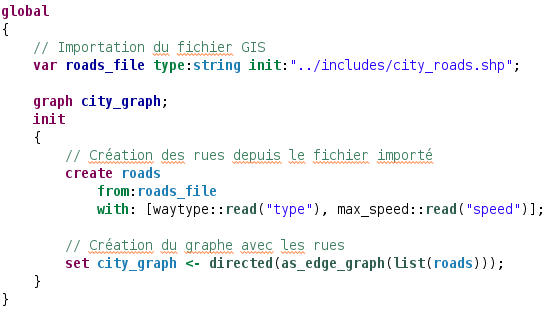
\includegraphics[width=\textwidth]{images/global-gaml.png}%
\end{center}
\caption{Initialisation des rues}%
\label{global}
\end{figure}%
Pour donner un aspect visuel \`a ces agents, il suffit \`a l'utilisateur d'en cr\'eer un nouveau type, h\'eritant des nôtres, et de lui d\'efinir ces propri\'et\'es (forme, couleur, taille), comme indiqu\'e dans la figure \ref{aspect}.
\begin{figure}[H]%
\begin{center}
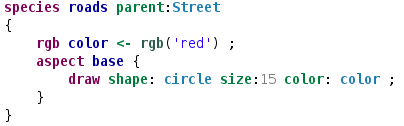
\includegraphics[width=0.77\textwidth]{images/aspect-gaml.png}%
\end{center}
\caption{H\'eritage de l'agent Street et red\'efinition de l'aspect}%
\label{aspect}
\end{figure}%


\subsection{Probl\`eme}
Les mouvements des agents sur le trac\'e est un parcours de graphe et l'algorithme de plus court chemin est impl\'ement\'e dans une librairie externe \`a GAMA. Se pose alors le probl\`eme de pouvoir reconstituer en m\'emoire un graphe \`a partir de nos informations relationnelles, alors que GAMA se base uniquement sur des coordonn\'ees des points pour g\'erer ses graphes.\\
On s'aperçoit alors de l'ampleur du travail pour permettre \`a cette approche de se concr\'etiser, surtout \'etant donn\'e le fait que le code Java de l'application est peu (voire pas) comment\'e ou document\'e. R\'ecup\'erer les \'el\'ements de l'API permettant l'impl\'ementation de notre solution impliquerait donc un temps encore plus important, sans compter le suppl\'ement \`a ajouter pour se familiariser \`a des nouvelles librairies pour l'ex\'ecution du parcours (style GraphStream).\\
Parall\`element, alors que nous commencions s\'erieusement \`a bloquer sur le probl\`eme, M. Nicolas MARILLEAU nous a envoy\'e un exemple de simulation o\`u les sens uniques sont g\'er\'es \`a l'aide du sens de digitalisation des points. Le traitement est effectu\'e enti\`erement en code GAML, ce qui implique l'existence de fonctions dans le code Java pour cela, fonctions que l'on pourra r\'eutiliser dans notre plug-in. Cet exemple nous a de plus clarifier le concept de sens de digitalisation (qui \'etait assez n\'ebuleux pour nous \`a la base) et le fonctionnement de GAMA pour ses parcours de graphe.

\section{Deuxi\`eme approche : \`a partir du sens de digitalisation des points}

\subsection{Avantages de la m\'ethode}
En effet, l'algorithme de parcours des graphes utilis\'e dans GAMA se base sur ce sens de digitalisation. Un test en GAML nous l'a confirm\'e : il existe une commande permettant de d\'eclarer le graphe comme \'etant orient\'e. Nous avons donc pu voir que les agents, apr\`es avoir utilis\'e cette commande, parcouraient le graphe dans le sens de digitalisation (nous avons effectu\'e ce test avec un trac\'e cr\'e\'e par nos soins dans un SIG et import\'e dans GAMA), alors qu'ils allaient indiff\'eremment dans les deux directions auparavant.\\
Le comportement de d\'eplacement inclus dans le skill \og moving \fg{} (dont on a d\'ej\`a parl\'e plus haut) prend donc d\'ej\`a en compte les graphes orient\'es, ce qui implique un gain de temps consid\'erable pour nous :
\begin{itemize}
 \item Nous n'aurons pas besoin d'\'ecrire l'algorithme de parcours de graphe, mais simplement \`a modifier la structure de ce dernier.
 \item De ce fait, on pourra g\'erer le probl\`eme directement dans nos agents pr\'ed\'efinis et nous pourrons donc nous passer de l'\'ecriture d'un \og skill \fg{} particulier pour g\'erer leurs mouvements.
\end{itemize}

\subsection{Probl\`eme pos\'e et solutions envisag\'ees}
Nouveau probl\`eme : en d\'eclarant le graphe comme \'etant orient\'e, les voies \`a double sens sont alors \'egalement consid\'er\'ees comme des sens uniques. Il nous faudra donc, dans le cas des double-sens, dupliquer l'agent repr\'esentant la route, inverser son sens de digitalisation et le rajouter \`a la population des routes (ce qui revient donc, en m\'emoire, \`a dupliquer une ar\^ete du graphe et de changer son orientation).\\
Cette op\'eration de duplication pouvait \^etre impl\'ement\'ee de plusieurs mani\`eres : soit elle se faisait directement \`a la construction des agents routes que nous avons fourni dans le plug-in (au moment de l'instanciation, on v\'erifie si l'agent est une route \`a double sens-unique, et le cas \'ech\'eant, on le duplique) soit \`a l'appel d'un \og statement \fg{} (mot-cl\'e du langage). Dans ce cas, l'id\'ee aurait \'et\'e de cr\'eer un nouveau \og statement \fg{}, qui prendrait la liste des agents routes en param\`etre et qui retournerait cette liste enrichie des duplicats n\'ecessaires au traitement des routes \`a double-sens.\\
M\^eme si cette derni\`ere solution aurait \'et\'e plus propre (l'utilisateur n'ayant pas forc\'ement envie de faire une simulation impliquant une probl\'ematique de sens uniques pourrait se passer de la duplication forc\'ee des routes \`a double-sens) , nous avons pr\'ef\'er\'e impl\'ementer la premi\`ere solution, d'une part pour une question de facilit\'e au niveau programmation (acc\`es direct aux propri\'et\'es de l'agent et \`a sa population pour y ajouter le duplicat) et d'autre part, \`a cause d'un cruel manque de documentation \`a ce sujet dans la documentation d\'eveloppeur de GAMA. 

\subsection{Côt\'e SIG}
Contrairement \`a la m\'ethode relationnelle, il n'existe plus le besoin d'avoir une information concernant les sens de direction dans une table, vu que ceux-ci sont les sens de digitalisation des trac\'es. En revanche, il est toujours n\'ecessaire d'indiquer pour chaque route si elle est \`a sens-unique (ou pas) et si le sens de digitalisation doit \^etre invers\'e (en cas d'erreur ou de changement de sens de circulation). Concr\`etement, cela se traduit par l'ajout d'un attribut \og waytype \fg{} dans la base de donn\'ees du fichier SIG, pouvant prendre la valeur 0 (double-sens), 1 (sens unique)  ou 2 (sens unique avec inversion du sens de digitalisation). Cette convention de nommage doit \^etre respect\'ee pour que notre plug-in puisse traiter les informations correctement.

\subsection{Côt\'e plug-in}
Nous avons pu garder la classe repr\'esentant les routes (StreetAgent) d\'evelopp\'ee lors de nos essais avec la m\'ethode relationnelle. En revanche, nous avons pu nous passer de la classe des agents repr\'esentant les services, \'etant donn\'e que son seul rôle \'etait de leur fournir un identifiant, ce que nous n'utilisons plus ici.\\
C'est donc dans la classe StreetAgent que s'effectue la duplication n\'ecessaire au traitement des routes au double sens. En effet, au moment o\`u l'on donne une valeur \`a l'attribut du type de route (le \og waytype \fg{}), nous v\'erifions d\'esormais la valeur de celui-ci et agissons en cons\'equent.
\begin{itemize}
 \item Si sa valeur vaut 1 : on ne fait rien, l'agent est une route \`a sens unique et sera trait\'e correctement dans l'algorithme de parcours de graphe de GAMA.
 \item Si sa valeur vaut 2 : on r\'ecup\`ere la g\'eom\'etrie (qui correspond \`a une liste ordonn\'ee de points) de l'agent, et on l'inverse (l'ordre de la liste correspondant au sens de digitalisation du trac\'e dans le SIG).
 \item Si sa valeur vaut 0 : l'id\'ee est de faire un clone de l'agent courant et d'en inverser la g\'eom\'etrie. Nous nous sommes frott\'es ici \`a un obstacle : les objets \og Agent \fg{} \'etant d\'eclar\'es comme immuables, nous n'avons pas pu cr\'eer une v\'eritable copie, puisqu'en Java, on ne peut que dupliquer la r\'ef\'erence sur un objet immuable et non l'objet en lui m\^eme. De fait, en voulant inverser la g\'eom\'etrie de la copie, nous inversions aussi la g\'eom\'etrie de l'objet courant. Pour pallier \`a ce probl\`eme, nous cr\'eons donc un nouvel agent, auquel on donne les m\^emes propri\'et\'es que l'agent courant (sauf, \'evidemment, sa g\'eom\'etrie que l'on inverse) et l'ajoutons dans la m\^eme population que lui.
\end{itemize}

\subsection{Côt\'e GAML}
Grâce \`a cette m\'ethode d'impl\'ementation, le tout est rest\'e transparent pour l'utilisateur qui \'ecrit sa simulation en GAML. En effet, pour que le sens de circulation soit bien pris en compte, il lui suffit juste d'utiliser nos agents pr\'ed\'efinis pour cr\'eer ses routes et de d\'eclarer le graphe de la ville comme orient\'e, la prise en compte du type de route s'effectuant \`a l'importation du fichier SIG.

\subsection{Et la cr\'eation d'un statement ?}
Comme nous l'avons signal\'e au d\'ebut de cette partie, nous avons song\'e \`a cr\'eer un mot cl\'e dans le langage (un ''statement'') qui permettrait de traiter la duplication des routes \`a double sens dans un autre endroit qu'\`a l'instanciation de celles-ci.\\
Lorsque nous avons commenc\'e \`a nous pencher sur l'approche par sens de digitalisation, nous avons tout de m\^eme tent\'e cette m\'ethode, mais avons rapidement \'et\'e bloqu\'e par des probl\`emes triviaux (comment renvoyer un type de donn\'ee dans le code GAML ou encore comment acc\'eder au contenu d'une liste pass\'ee en param\`etre dans le code GAML dans le code Java). Autrement dit, cette m\'ethode s'est rapidement sold\'ee par un \'echec et par une perte de temps assez cons\'equente.

\chapter{Limitations de vitesse}
Deuxi\`eme \'etape de nos d\'eveloppement, nous nous sommes pench\'es sur les limitations de vitesse et de la vitesse d'un agent sur un tronçon, afin de mod\'eliser les engorgements.

\section{Objectif}
Nous voulions permettre aux utilisateurs du plug-in de d\'efinir une vitesse maximum \`a laquelle les agents rouleront sur un tronçon. Ensuite, en fonction du nombre d'agent circulant dans le m\^eme sens sur ce tronçon, la vitesse effective de chaque agent diminuerait en fonction d'une formule donn\'ee.

\section{Organisation du d\'eveloppement}
Dans un premier temps, nous avons cherch\'e \`a affecter une vitesse maximum \`a un tronçon et de faire rouler les agents \`a cette vitesse. Cette premi\`ere \'etape serait la plus dure car elle n\'ecessitait de mettre une pond\'eration sur un rue, et donc un arc du graphe. Ensuite les agents empruntant cette arc utiliseraient cette pond\'eration automatiquement, grâce aux algorithmes sur les graphes utilis\'es par GAMA.\\
La seconde \'etape consistait \`a ajouter un nouveau facteur : le nombre d'agent sur le tronçon. Deux approches ont \'et\'e trouv\'ee : l'une bas\'ee sur une attente active et l'autre sur une attente passive. Une fois le nombre d'agent obtenu, il suffisait d'appliquer une formule pour red\'efinir la nouvelle vitesse maximum.\\
Enfin, derni\`ere \'etape, nous voulions laisser l'utilisateur libre du choix de la formule, qu'il entrerait dans son fichier GAML et qui serait utilis\'ee par notre plug-in.

\section{Premi\`ere \'etape : Affecter la vitesse maximum}
Toujours pour simplifier la mod\'elisation de la ville, nous avons choisi de rajouter une nouvelle information \`a fournir dans le fichier SIG : la vitesse maximum sur la rue. Ainsi, l'utilisateur ne devra pas manuellement affecter la vitesse \`a chaque rue. Pass\'e cette formalit\'e, l'agent pr\'ed\'efini des rues que nous avons d\'evelopp\'e devait affecter cette valeur \`a l'arc qu'il repr\'esente dans le graphe.\\
H\'elas, deux facteurs nous ont emp\^ech\'es d'arriver au terme de cette tâche. D'une part,  nous n'avons pas r\'eussi \`a obtenir l'arc du graphe correspondant \`a une rue a cause du fonctionnement interne complexe de GAMA. D'autre part, le temps imparti aux projet tuteur\'es arrivait \`a son terme.

\section{Seconde \'etape : Le nombre d'agent sur le tronçon}
Malgr\'e la fin du d\'eveloppement, nous avions tout de m\^eme quelques id\'ees pour l'impl\'ementation de cette partie : un m\'ethode active et une m\'ethode passive.

\subsection{La m\'ethode active}
La m\'ethode active \'etait fort simple : boucler ind\'efiniment sur une r\'ecup\'eration de tous les agents, puis le calcul de la vitesse et la modification du poids de l'ar\^ete. Comme toutes les m\'ethodes actives, elle n'est pas tr\`es optimis\'ee puisque le calcul est effectu\'e, qu'il y ait des agents ou non. Il serait plus int\'eressant de ne faire le calcul qu'\`a l'entr\'ee ou la sortie d'un agent dans la rue.

\subsection{La m\'ethode passive}
L'id\'ee \'etait donc qu'un agent devrait signaler \`a la rue qu'il va entrer ou sortir de celle-ci. Ainsi, on peut stocker le nombre d'agents dans la rue et ne recalculer la vitesse que lorsqu'il le faut.

\section{Troisi\`eme \'etape : G\'en\'eralisation de la formule}
Jusqu'ici nous utilisions une formule, $v = v_{max} *  ( 1 -\frac{n}{k})$ , avec, $v_{max}$ la vitesse maximum sur la rue, $n$ le nombre d'agent sur la rue et $k$ le nombre d'agent maximum sur la rue. Celle-ci serait jusque l\`a inscrite en dur dans l'agent pr\'ed\'efini symbolisant les rues. L'utilisateur ne pourrait donc pas utiliser la sienne, m\^eme si elle \'etait plus pertinente.\\
Nous voulions donc laisser aux utilisateurs la possibilit\'e de renseigner leurs propres formules dans le code GAML, mais n'ayant pas dej\`a pu mettre en place la formule \`a temps, nous n'avons pas du tout \'etudi\'e cette fonctionnalit\'e.

\chapter{Le plug-in final}
La derni\`ere version du plug-in \`a ce jour permet donc de cr\'eer un mod\'elisation de base pour une ville. D'un part des rues sur lesquelles les agents roulent et respectent les sens-uniques. Elles peuvent \^etre g\'en\'er\'ees depuis un fichier SIG et on peut leur d\'efinir une vitesse maximum mais celle-ci n'est pas utilis\'ee par les agents. Et d'autre part, des services symbolisant les intersections, les points de d\'epart et les points d'arriv\'ees des agents circulant dans la ville.\\
Notre principale difficult\'e fut la complexit\'e de la plateforme GAMA. Beaucoup de temps et d'\'energie furent d\'epens\'es pour mettre en place un simple graphe orient\'e et quand bien m\^eme celui-ci fonctionnât, nous n'avons pas pu l'adapter pour g\'erer la vitesse des agents.\\
Un sentiment de frustration g\'en\'erale a donc \'et\'e ressenti tout au long de notre travail sur ce projet (surtout au niveau du ratio temps de travail / r\'esultats obtenus)  m\^eme si nous avons pu compter sur l'aide de nos tuteurs pour nous r\'e-aiguiller vers d'autres pistes pour r\'esoudre nos probl\`emes. L'aspect positif de ceci (parce qu'il en faut bien un) aura \'et\'e la constante remise en question de la conception de nos fonctionnalit\'es impliqu\'ee.

\end{document}

